\definecolor{c3}{RGB}{41 160 203}
\definecolor{c4}{RGB}{231 138 195}
\definecolor{c5}{RGB}{92 53 102}
\definecolor{c6}{RGB}{252 233 79}



% GNUPLOT: LaTeX picture with Postscript
\begingroup
  \makeatletter
  \providecommand\color[2][]{%
    \GenericError{(gnuplot) \space\space\space\@spaces}{%
      Package color not loaded in conjunction with
      terminal option `colourtext'%
    }{See the gnuplot documentation for explanation.%
    }{Either use 'blacktext' in gnuplot or load the package
      color.sty in LaTeX.}%
    \renewcommand\color[2][]{}%
  }%
  \providecommand\includegraphics[2][]{%
    \GenericError{(gnuplot) \space\space\space\@spaces}{%
      Package graphicx or graphics not loaded%
    }{See the gnuplot documentation for explanation.%
    }{The gnuplot epslatex terminal needs graphicx.sty or graphics.sty.}%
    \renewcommand\includegraphics[2][]{}%
  }%
  \providecommand\rotatebox[2]{#2}%
  \@ifundefined{ifGPcolor}{%
    \newif\ifGPcolor
    \GPcolorfalse
  }{}%
  \@ifundefined{ifGPblacktext}{%
    \newif\ifGPblacktext
    \GPblacktexttrue
  }{}%
  % define a \g@addto@macro without @ in the name:
  \let\gplgaddtomacro\g@addto@macro
  % define empty templates for all commands taking text:
  \gdef\gplfronttext{}%
  \gdef\gplfronttext{}%
  \makeatother
  \ifGPblacktext
    % no textcolor at all
    \def\colorrgb#1{}%
    \def\colorgray#1{}%
  \else
    % gray or color?
    \ifGPcolor
      \def\colorrgb#1{\color[rgb]{#1}}%
      \def\colorgray#1{\color[gray]{#1}}%
      \expandafter\def\csname LTw\endcsname{\color{white}}%
      \expandafter\def\csname LTb\endcsname{\color{black}}%
      \expandafter\def\csname LTa\endcsname{\color{black}}%
      \expandafter\def\csname LT0\endcsname{\color[rgb]{1,0,0}}%
      \expandafter\def\csname LT1\endcsname{\color[rgb]{0,1,0}}%
      \expandafter\def\csname LT2\endcsname{\color[rgb]{0,0,1}}%
      \expandafter\def\csname LT3\endcsname{\color[rgb]{1,0,1}}%
      \expandafter\def\csname LT4\endcsname{\color[rgb]{0,1,1}}%
      \expandafter\def\csname LT5\endcsname{\color[rgb]{1,1,0}}%
      \expandafter\def\csname LT6\endcsname{\color[rgb]{0,0,0}}%
      \expandafter\def\csname LT7\endcsname{\color[rgb]{1,0.3,0}}%
      \expandafter\def\csname LT8\endcsname{\color[rgb]{0.5,0.5,0.5}}%
    \else
      % gray
      \def\colorrgb#1{\color{black}}%
      \def\colorgray#1{\color[gray]{#1}}%
      \expandafter\def\csname LTw\endcsname{\color{white}}%
      \expandafter\def\csname LTb\endcsname{\color{black}}%
      \expandafter\def\csname LTa\endcsname{\color{black}}%
      \expandafter\def\csname LT0\endcsname{\color{black}}%
      \expandafter\def\csname LT1\endcsname{\color{black}}%
      \expandafter\def\csname LT2\endcsname{\color{black}}%
      \expandafter\def\csname LT3\endcsname{\color{black}}%
      \expandafter\def\csname LT4\endcsname{\color{black}}%
      \expandafter\def\csname LT5\endcsname{\color{black}}%
      \expandafter\def\csname LT6\endcsname{\color{black}}%
      \expandafter\def\csname LT7\endcsname{\color{black}}%
      \expandafter\def\csname LT8\endcsname{\color{black}}%
    \fi
  \fi
    \setlength{\unitlength}{0.0500bp}%
    \ifx\gptboxheight\undefined%
      \newlength{\gptboxheight}%
      \newlength{\gptboxwidth}%
      \newsavebox{\gptboxtext}%
    \fi%
    \setlength{\fboxrule}{0.5pt}%
    \setlength{\fboxsep}{1pt}%
\begin{picture}(5000.00,1600.00)%
    \gplgaddtomacro\gplfronttext{%
      \colorrgb{0.15,0.15,0.15}%
      \put(468,160){\makebox(0,0)[r]{\strut{}\scriptsize $10^{-1}$}}%
      \colorrgb{0.15,0.15,0.15}%
      \put(368,586){\makebox(0,0)[r]{\strut{}\scriptsize $10^{0}$}}%
      \colorrgb{0.15,0.15,0.15}%
      \put(468,1013){\makebox(0,0)[r]{\strut{}\scriptsize $10^{+1}$}}%
      \colorrgb{0.15,0.15,0.15}%
      \put(468,1439){\makebox(0,0)[r]{\strut{}\scriptsize $10^{+2}$}}%
      \colorrgb{0.15,0.15,0.15}%
      \put(500,-60){\makebox(0,0){\strut{}\scriptsize $10^0$}}%
      \colorrgb{0.15,0.15,0.15}%
      \put(959,-60){\makebox(0,0){\strut{}\scriptsize $10^{+1}$}}%
      \colorrgb{0.15,0.15,0.15}%
      \put(1419,-60){\makebox(0,0){\strut{}\scriptsize $10^{+2}$}}%
      \colorrgb{0.15,0.15,0.15}%
      \put(1878,-60){\makebox(0,0){\strut{}\scriptsize $10^{+3}$}}%
    }%
    \gplgaddtomacro\gplfronttext{%
      \colorrgb{0.15,0.15,0.15}%
      \put(1349,-390){\makebox(0,0){\strut{}\footnotesize Area [m$^2$]}}%
      \colorrgb{0.00,0.00,0.00}%
      \put(1349,1859){\makebox(0,0){\strut{}\footnotesize Execution time vs area}}%
      \put(1100,1600){\makebox(0,0){\strut{}{\color{c3}{\rule[0.6mm]{0.3cm}{0.5mm}}} \scriptsize FastVGICP}}
      \put(1900,1600){\makebox(0,0){\strut{}{\color{c4}{\rule[0.6mm]{0.3cm}{0.5mm}}} \scriptsize \texttt{x1}}}
      \put(3500,1600){\makebox(0,0){\strut{}{\color{c5}{\rule[0.6mm]{0.3cm}{0.5mm}}} \scriptsize t minus \texttt{sm2}}}
      \put(4600,1600){\makebox(0,0){\strut{}{\color{c6}{\rule[0.6mm]{0.3cm}{0.5mm}}} \scriptsize Intersections}}
    }%
    \gplgaddtomacro\gplfronttext{%
      \colorrgb{0.15,0.15,0.15}%
      \put(2993,160){\makebox(0,0)[r]{\strut{}\scriptsize $0.0$}}%
      \colorrgb{0.15,0.15,0.15}%
      \put(2993,416){\makebox(0,0)[r]{\strut{}\scriptsize $0.2$}}%
      \colorrgb{0.15,0.15,0.15}%
      \put(2993,672){\makebox(0,0)[r]{\strut{}\scriptsize $0.4$}}%
      \colorrgb{0.15,0.15,0.15}%
      \put(2993,927){\makebox(0,0)[r]{\strut{}\scriptsize $0.6$}}%
      \colorrgb{0.15,0.15,0.15}%
      \put(2993,1183){\makebox(0,0)[r]{\strut{}\scriptsize $0.8$}}%
      \colorrgb{0.15,0.15,0.15}%
      \put(2993,1439){\makebox(0,0)[r]{\strut{}\scriptsize $1.0$}}%
      \colorrgb{0.15,0.15,0.15}%
      \put(3025,-60){\makebox(0,0){\strut{}\scriptsize $10^0$}}%
      \colorrgb{0.15,0.15,0.15}%
      \put(3506,-60){\makebox(0,0){\strut{}\scriptsize $10^{+1}$}}%
      \colorrgb{0.15,0.15,0.15}%
      \put(3987,-60){\makebox(0,0){\strut{}\scriptsize $10^{+2}$}}%
      \colorrgb{0.15,0.15,0.15}%
      \put(4468,-60){\makebox(0,0){\strut{}\scriptsize $10^{+3}$}}%
      \colorrgb{0.15,0.15,0.15}%
      \put(4949,-60){\makebox(0,0){\strut{}\scriptsize $10^{+4}$}}%
    }%
    \gplgaddtomacro\gplfronttext{%
      \colorrgb{0.15,0.15,0.15}%
      \put(3987,-390){\makebox(0,0){\strut{}\footnotesize Area [m$^2$]}}%
      \colorrgb{0.00,0.00,0.00}%
      \put(3987,1859){\makebox(0,0){\strut{}\footnotesize Timing breakdown vs area}}%
    }%
    \put(0,0){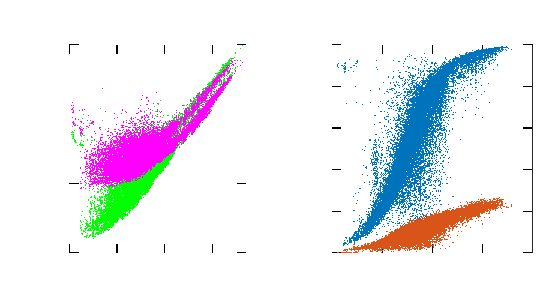
\includegraphics{./figures/experiments/c/time_analysis}}%
    \gplfronttext
  \end{picture}%
\endgroup
